%\documentclass[xcolor=svgnames]{beamer}
%\includeonlyframes{current}


\documentclass[xcolor=svgnames,handout]{beamer}

\usepackage{MnSymbol,wasysym}
\usepackage[utf8]    {inputenc}
\usepackage[T1]      {fontenc}
\usepackage[english] {babel}

\usepackage{amsmath,amsfonts,graphicx}
\usepackage{beamerleanprogress}
\usepackage{xcolor}
\usepackage{soul}
%\usepackage{verbatim}
\usepackage{multicol}
\usepackage{tikz} 
\usepackage[export]{adjustbox}
\usepackage{verbatim}

\definecolor{iyellow}{RGB}{255, 162, 23}
\definecolor{sgreen}{RGB}{118, 191, 138}

\newcommand{\yellow}[1]{\textcolor{iyellow}{#1}}
\newcommand{\orange}[1]{\textcolor{OrangeRed}{#1}}
\newcommand{\green}[1]{\textcolor{sgreen}{#1}}
\newcommand{\red}[1]{\textcolor{red}{#1}}
\newcommand{\blue}[1]{{\textcolor{blue}{#1}}}
%\newcommand{\newpt}{\par \vspace{5mm}}

\newcommand{\cell}[1]{{\sf \textbf{\textcolor{DarkMagenta}{#1}}}}
\newcommand{\ft}[1]{\frametitle{#1}}
\newcommand{\ra}{$\rightarrow$ }
\newcommand{\eol}{\\[1em]\pause}

\usepackage[T1]{fontenc}
\usepackage[utf8]{inputenc}
\usepackage{tikz}
\usetikzlibrary{shadows}

\newcommand*\keystroke[1]{%
  \tikz[baseline=(key.base)]
    \node[%
      draw,
      fill=white,
      drop shadow={shadow xshift=0.25ex,shadow yshift=-0.25ex,fill=black,opacity=0.75},
      rectangle,
      rounded corners=2pt,
      inner sep=1pt,
      line width=0.5pt,
      font=\scriptsize\sffamily
    ](key) {#1\strut}
  ;
}

\title
  [Data 301 Data Analytics\hspace{2em}]
  {Data 301 Data Analytics\\
Microsoft Execl VBA}

\author
  [Dr.\ Irene Vrbik]
  {Dr.\ Irene Vrbik}

\date
  {Term 1, 2018}

\institute
  {University of British Columbia Okanagan \newline irene.vrbik@ubc.ca}


\graphicspath{{img/}}

\begin{document}

\maketitle

\setbeamersize{description width=0.57cm} % to have less indent with the description environment

\section{Creating Macros}


\frame{
\ft{What is VBA?}

Excel Visual Basic for Applications (VBA)

Visual Basic for Applications (VBA) is a programming language developed by Microsoft\eol

It allows users to build their own functions, automate tasks in Microsoft Office, and develop customized code.\eol

The language has been part of almost all versions of Office for over 20 years.\eol

VBA allows for expanding the capabilities of Excel and adding user-interface elements (buttons, lists) to your spreadsheet.

}

\begin{frame}
  {Why Microsoft Excel Visual Basic for Applications?}
Microsoft Excel VBA allows for automating tasks in Excel and provides a full programming environment for data analysis.\pause
\begin{itemize}
\item We can use VBA to automate tedious processes in Excel, eg. formatting a month report\eol
\end{itemize}

Excel VBA is commonly used in high finance and frequency trading applications for creating and validating financial models.\eol

Using Excel VBA will be our first practice with programming and allow us to explore fundamental programming concepts of commands, variables, decisions, repetition, objects, and events.
\end{frame}

\frame{
\ft{Macros}
A macro is a recorded set of actions that is saved so that they can be easily executed again.\eol

If you do the same set of actions repetitively, then creating a macro allows for doing all those actions with one command.\eol
Macros are accessible under the {\bf View} tab in the {\bf Macros} group or the {\bf Developer} tab.\eol

Macros are converted into VBA programs.  
}
%A macro (short for "macroinstruction", from Greek ?????? 'long') in computer science is a rule or pattern that specifies how a certain input sequence (often a sequence of characters) should be mapped to a replacement output sequence (also often a sequence of characters) according to a defined procedure. The mapping process that instantiates (transforms) a macro use into a specific sequence is known as macro expansion. 

\frame{
\ft{Developer Tab}
The Developer tab contains icons for performing VBA and macro development.  \eol

This tab is disabled by default.\eol

To add the Development tab on a PC, go to File, Options, Customize Ribbon and make sure it is checked beside Developer.\eol

For a Mac, go to {\bf Excel}, {\bf Preferences}, {\bf View}.  Under the  \textit{In Ribbon, Show} heading, select the checkbox marked ``Developer Tab"

}

\frame[label=current]{
\ft{Recording a Macro }



To record a macro, go to the {\bf View} tab and select  the ``Record Macro'' button 
\begin{onlyenv}<1-5>
  \begin{center}
  \includegraphics<2->[width=2em]{img/recordmacro.png}
    \includegraphics<5->[width=0.4\textwidth]{img/ReservedShortcut}
  \end{center}
\end{onlyenv}
\uncover<3->{Macro names cannot contain spaces or begin with a number.}\eol
\uncover<4->{It is recommended to use \keystroke{Ctrl}+\keystroke{Shift}+{\tt <Key>} (PC)/\keystroke{Option}+\keystroke{Cmd}+{\tt <Key>} (Mac) for a Shortcut key so that you do not override built-in shortcuts.}\uncover<5->{Macs will give you a warning when you attempt to override an existing shortcut}\eol
\uncover<6->{A macro can be created without assigning it a shortcut key.}

} 

\frame[t]{
As a simple example, we could create a macro that bold and italicizes a cell.
$$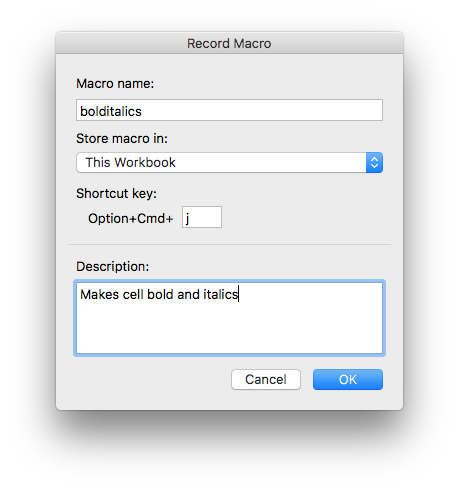
\includegraphics[width=0.5\textwidth]{img/bolditalics}$$

Excel will record your actions until you select {\bf Stop Recording}.
\begin{itemize}
\item Note: Cursor movement is not captured.
\end{itemize}
}


\frame{
\ft{Recording Macros}
By default, macros are created using absolute references %({\tt $A$1} rather than {\tt A1}
\begin{itemize}
\item To use Relative references, we need turn on the ``Use Relative References" button, \underline{before} we record.
\end{itemize}
While the Macro Recorder makes creating macros very easy, it has it's limitations:
\begin{itemize}
\item \alert{\frownie{}\frownie{} There is no way (that I can find) to do this on a Mac \frownie{}\frownie{}}
\item eg. cannot handle ``loops" (more on loops later)
\item generates more code than is necessary (which can slow down your process).
\end{itemize}
For that reason, we better learn some code \dots
}


%\begin{frame}
%But first, ... 
%A) A macro can be created without assigning it a shortcut key.
%B) A macro will record cursor movements.
%C) Macros can be created in an individual workbook or in a personal macro workbook so they can be used in multiple workbooks.
%D) A macro can have only one command it executes.
%\end{frame}


\section{Using Macros}

\frame{
\ft{Using a Macro}
There are a number of ways you can use your macro:
\begin{enumerate}
\item With the shortcut key if defined
\item Under {\bf Macros}, Select {\bf View Macros} then pick the macro and {\bf Run}.
\item Assign a macro to a button or on the toolbar
\end{enumerate}
}

\frame[t]{
\ft{Macro Buttons}
To assign a macro button:
\begin{enumerate}

\item Select the {\bf Developer} tab and click 
$$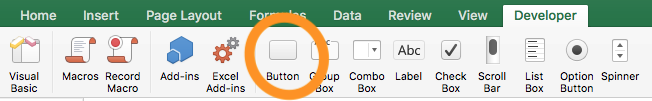
\includegraphics[height=3.5em]{img/button.png}.$$
\item To prompt the Assign Macro popup window, click where you would like this button to appear on your worksheet.
\begin{itemize}
\item Note: If you have already inserted a button (eg. {\bf Insert} "Shapes"), you can right-click on it, and select {\bf Assign Macro}.
\end{itemize}
\item Assign a macro to the button by selecting one from the list of existing macros or creating a brand new one and click OK.
%\item To specify the control properties of the button, right-click it, and then select Format Control....
\end{enumerate}
}

\frame{
\ft{Macro Toolbars}
To add a macro to The Quick Access Toolbar, select:
\begin{enumerate}
\item \begin{description}
\item[PC] {\bf File} \ra {\bf Options} \ra \textit{Quick Access Toolbar}.
\item[Mac] {\bf Excel} \ra {\bf Preferences} and click \textit{Ribbon and Toolbar} \ra \textit{Quick Access Toolbar} header
\end{description}
\item In the ``Choose commands" drop-down menu, select {\bf Macros}
\item Select the macro and add to your toolbar (click this 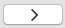
\includegraphics[width=2em]{img/add.png})
\item  Modify the button with a unique symbol (eg. \smiley{}).
\begin{itemize}
\item \frownie{}\frownie{} Feature not available on a mac? \frownie{}\frownie{}
\end{itemize}
\end{enumerate}
}

\begin{frame}[fragile]
\ft{Macro Buttons}
You can assign multiple macros to a single button!
To assign multiple macro button:

\begin{enumerate}
\item Select the {\bf Developer} tab and click 
$$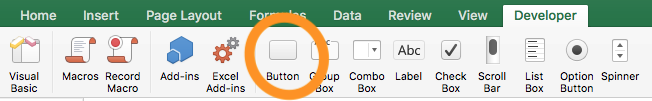
\includegraphics[height=3.5em]{img/button.png}.$$
\item To prompt the Assign Macro popup window, click where you would like this button to appear on your worksheet.
\item Select "New" and the VBA editor will open. Type the name of the macros you wish to assign in the body of the Sub.
\begin{verbatim}
  Sub ButtonX_Click() 
      bolditalics
      UNDERLINE
  End Sub
\end{verbatim}
\end{enumerate}
\end{frame}


\begin{frame}
\ft{Try It: Macros}
\begin{exampleblock}{Question}
Create a macro that does the following tasks:
\begin{enumerate}
\item Use a shortcut of \keystroke{Ctrl}+\keystroke{Shift}+\keystroke{b} (PC)/\keystroke{Opt}+\keystroke{Cmd}+\keystroke{b} (Mac).
\item Bolds the cell and makes the font Courier 20
\item Sets the cell background to orange.
\item Centers the text in the cell.
\item Add it to a button in the shape of a star that says OC20
\end{enumerate}
\end{exampleblock}
Try-out your macro using 1) the shortcut key, 2) the macro dialog, and 3) the macro button, and 
\end{frame}



\section{Saving}
\frame{
\ft{Saving macros}
In order to save the workbook with the macros we've created while it was open, we need  use a  "macro-enabled" file format.\eol
When you go to save a workbook containing macros, you will receive the following popup
$$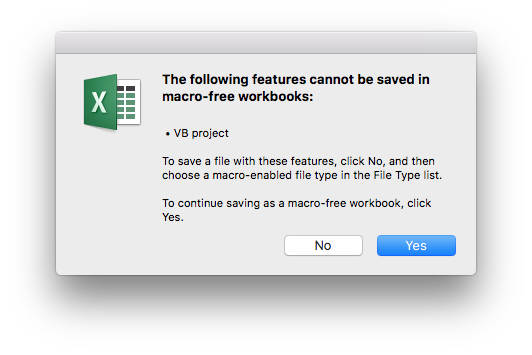
\includegraphics[width=0.5\textwidth]{img/SavingMacro.png}$$
\vspace{-2em}
\begin{itemize}
\item  `Yes' will save it as as macro-enabled workbook (*.xlsm file)
\item  `No' will save it as as macro-free workbook (*.xlsx file)
\end{itemize}

}

\frame{
\ft{Saving macros}
Saving a macros to a  given workbook will only allow you to use it with that file.\eol
We could alternatively save it to a \emph{Personal Workbook} allowing them to be used in multiple workbooks.\eol
Your Personal Workbook is a hidden workbook saved under the name {\bf personal.xlsb}\eol
This file loads every time you open up excel \eol
Hence saving a macro to {\bf personal.xlsb} will allow you to use that macro on any workbook that you open on your computer
}


\frame{
\ft{Saving macros}
To save it to your personal workbook,  select the "Personal Macro Workbook" option in the drop-down menu for "Store Macro in"
$$
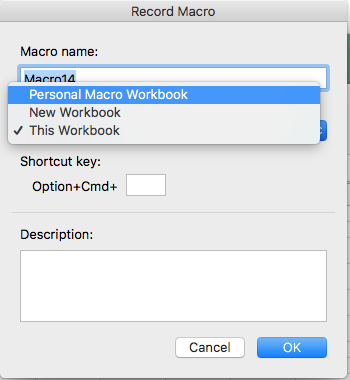
\includegraphics[width=0.4\textwidth]{img/PWB.png}$$
}


\frame{
\ft{Macro Security}
Since macros can execute any code, they have been a target for virus writers.  \eol
Understanding the source of the Excel spreadsheet that contains macros is important when deciding to run them or not.\eol

Excel has \emph{macro security settings} to allow you to enable or disable running macros.  \eol

Spreadsheets with macros often will generate a warning when opening them:
$$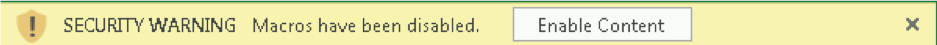
\includegraphics[width=0.9\textwidth]{img/security}$$
}

\frame{
\ft{Macro Security Settings}
The default security is  to \emph{Disable all macros with notification}. This prevents macros from running but displays a warning allowing you to enable them.\eol
One of the biggest issues with macros is security\eol
Make sure you are only using macros from a trusted source.\eol

On the {\bf Developer} tab, click "Macro Security" located below the "Record Macro" button.  Select a desired option in Macro Settings category, under the \textit{Macro Settings} header (PC)/ or in {\bf Excel} \ra {\bf Preference} "Security \& Privacy"\eol

\begin{tikzpicture}[remember picture,overlay]%[xshift=65mm,yshift=-48mm,anchor=north west]
\node at (current page.center) {\includegraphics<handout:0| beamer:5>[width=.7\textwidth]{img/securityPC}};
\end{tikzpicture}
\begin{tikzpicture}[remember picture,overlay]%[xshift=65mm,yshift=-48mm,anchor=north west]
\node at (current page.center) {\includegraphics<handout:0| beamer:6>[width=.7\textwidth]{img/securityOpts}};
\end{tikzpicture}
}



\frame{
\ft{Macros: Implementation}
Macros are converted to Visual Basic code.\eol

You can edit macro code and create your own code.\eol

Under the Developer tab, select Macros then Edit macro to modify the code.\eol

The code will then open in you \emph{Visual Basic Editor (VBE)}\eol
 It is best practice to break long tasks  into, smaller relevant macros rather than one big macro.\eol
 Macros can be written for and any other Office application that supports VBA. \pause


}

\frame{
\ft{Visual Basic Editor}
Visual Basic Editor (VBE) allows editing visual basic code and is a complete integrated development environment (IDE).\eol

Users can create and edit macros as well as other Visual Basic code with the editor.\eol

To open the VBE, under {\bf Developer} tab \ra {\bf Visual Basic} or \keystroke{Alt}+\keystroke{F11} (PC)/ \keystroke{Opt}+\keystroke{F11} (Mac).\eol

There is also a quick button for this in the left hand side of the Developer tab:
$$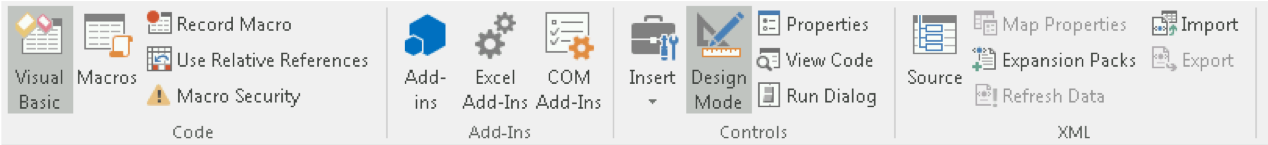
\includegraphics[width=0.8\textwidth]{img/VBE}$$
}

\frame{
\ft{Visual Basic Edior}
$$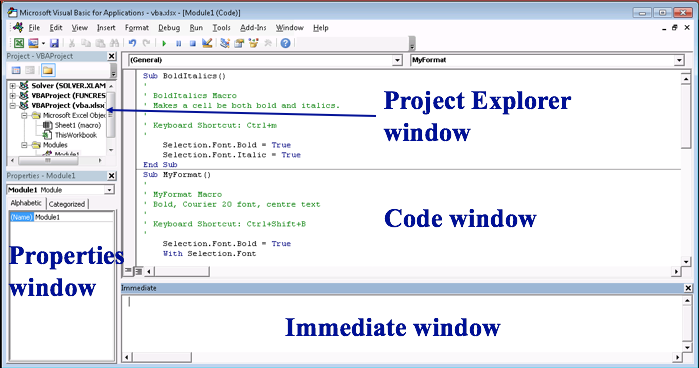
\includegraphics[width=0.9\textwidth]{img/VBEwindow}$$
}

\frame{
\ft{Object Browser}
\emph{Object browser} allows for exploring objects and methods (the application programming interface (API)) of Excel VBA.  Open with \keystroke{F2}.
$$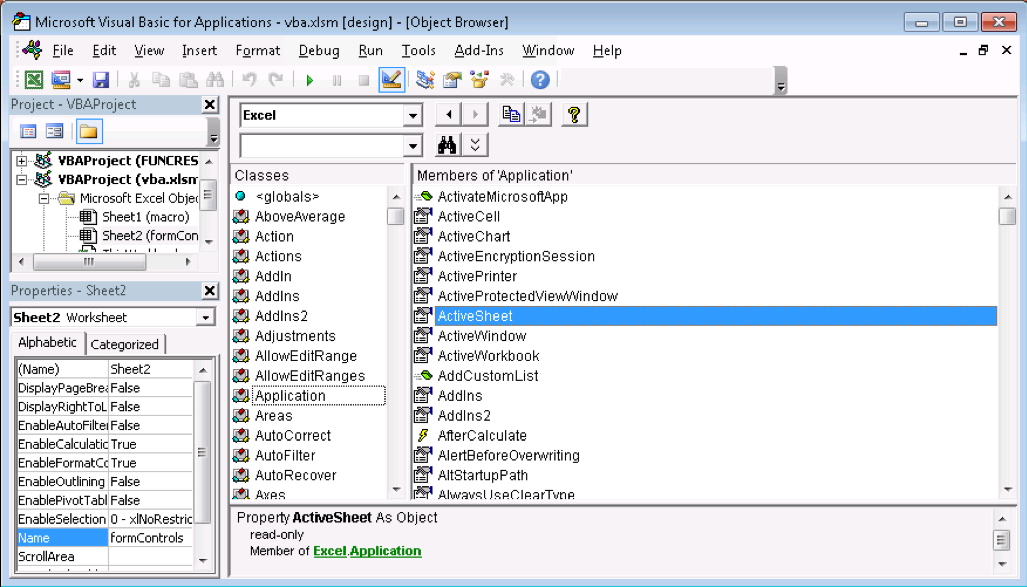
\includegraphics[width=0.9\textwidth]{img/ObjectBrowser}$$
}


\frame{
\ft{Macro Code in Visual Basic Editor}
$$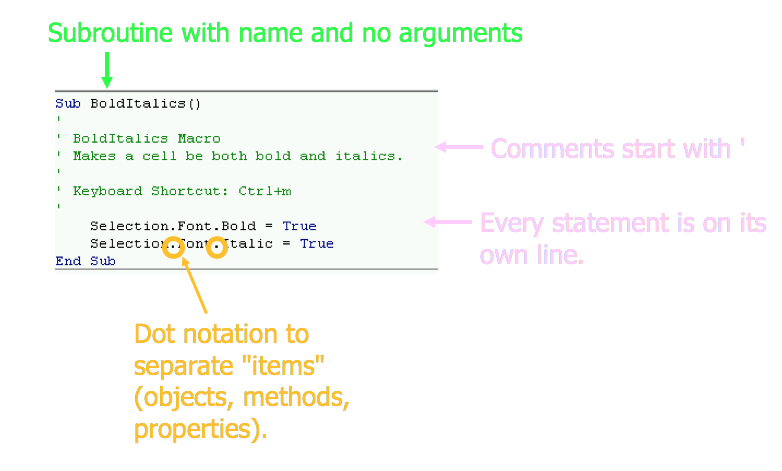
\includegraphics[width=0.99\textwidth]{img/MacroCode}$$
}

\frame{
\ft{{\tt} WITH Statement in Visual Basic Code}
$$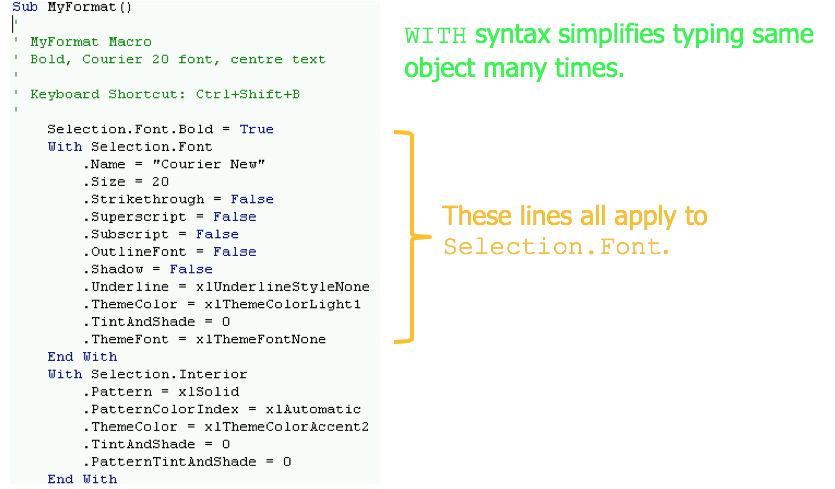
\includegraphics[width=0.99\textwidth]{img/with}$$
}

\frame{
\ft{Visual Basic Editor: Immediate Window}
The Immediate window allows entering of single line commands.
\begin{itemize}
\item Use {\tt PRINT} or {\tt?}
\item In code, use {\tt Debug.Print} to print to immediate window.
\end{itemize}
$$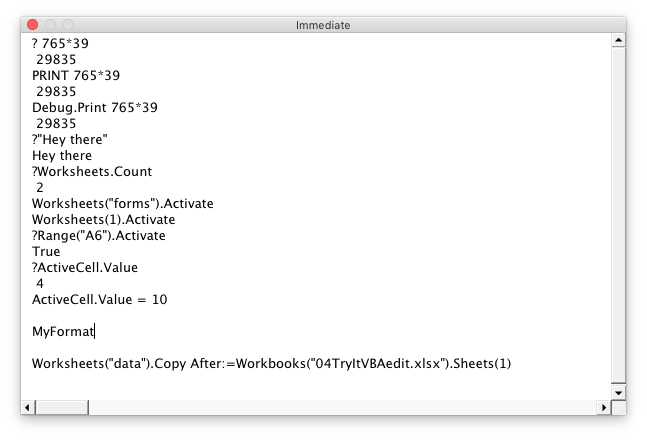
\includegraphics[width=0.8\textwidth]{img/immediate}$$
}

\frame{
\ft{Try It: Immediate Window}
\begin{exampleblock}
{Question:} Try do these actions using the immediate window:
\begin{enumerate}
\item Print {\tt "Hey There!"}
\item Calculate the answer of 765 * 39.
\item Select a cell then call the macro RedItalics.
\item Change the value of cell B4 to "DATA".
\item Change the value of cell A6 to 100.
\end{enumerate}
\end{exampleblock}
}

\frame{
\ft{Challenge Try it: Create a Macro in VBE}
\begin{exampleblock}
{Question} Copy the MyFormat macro and edit to produce a new macro called RedUnderline that:
Underlines the text in the cell.
Makes the cell background red.
If the cell was bold or italics before, resets to not have bold and italics.
\end{exampleblock}

Hints:
\begin{itemize}
\item Underline property in Excel is {\tt Font.Underline} and can set to constant {\tt xlUnderlineStyleSingle}.
\item Can change background color with {\tt Interior.Color} and set to {\tt RGB(redValue, greenValue, blueValue)} where the colour values are numbers from 0 to 255.
\end{itemize}
}


\frame{
\ft{Introduction to Programing}
An \emph{algorithm} is a precise sequence of steps to produce a result.  A program is an encoding of an algorithm in a \emph{language} to solve a particular problem.\eol

There are numerous languages that programmers can use to specify instructions.  Each language has its different features, benefits, and usefulness.\eol

We will start with Excel VBA but also study Python and R.\eol

The goal is to understand fundamental programming concepts that apply to all languages.
}

\begin{frame}[fragile]
\frametitle{Variables}
A \emph{variable} is a name that refers to a location that stores a data value.
$$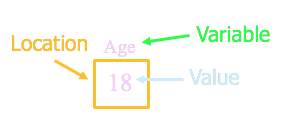
\includegraphics[width=0.4\textwidth]{img/Variable}$$
\begin{alert}
{IMPORTANT:} The \emph{value} at a location can change using initialization or assignment.\eol
\end{alert}
\emph{Assignment} using an  sets the value of a variable.\eol
Example:
\begin{itemize}
\item 
\begin{verbatim}
num = 10
num = Range("A1").Value
\end{verbatim}
\end{itemize}
\end{frame}

\begin{frame}[fragile]
\ft{Excel Variables}
Every variable in Excel has a \emph{name} and a \emph{data type}.\eol
Variables increase code efficiency and readability.\eol
Data types: Boolean, Currency, Date, Double, Integer, Long, Object, String, Variant (any type)\eol
Example:
\begin{itemize}
\item 
{\tt \yellow{Dim} num \yellow{As Integer}}
\end{itemize}
\end{frame}
% https://www.excelfunctions.net/vba-variables-and-constants.html
%From the above table, it is clear that you can save on memory by using specific data types (e.g. Integers rather than Longs, or Singles rather than Doubles). However, if you are planning to use the 'smaller' data types, you must be sure that your code will not encounter larger values than can be handled by the chosen data type.

\begin{frame}[fragile]
\ft{Collections}
\emph{Collections} are variables that store multiple data items. \eol

Data items can either be indexed (selected) by name or number.\eol
Example:
\begin{itemize}
\item 
\begin{verbatim}
Worksheets("macro")
Worksheets(2)
\end{verbatim}
\end{itemize}
{\tt Worksheets} is a collection as there may be multiple worksheets in the workbook.  Select one by name or number (starting with 1).
\end{frame}

\begin{frame}[fragile]
\ft{Variables Question}
\begin{exampleblock}
{Question} How many of the following statements are TRUE?
\begin{enumerate}
\item A variable name cannot change during a program.
\item A variable value cannot change during a program.
\item A collection is a variable that can store multiple data items.
\item A value in a collection can be retrieved by name or by index starting from 0.
\item In Excel, variables are declared using DIM.
\item In Excel, variables are declared with a data type.
\end{enumerate}
\begin{multicols}{5}
\begin{enumerate}[A)]
\item 0 
\item 1
\item 2
\item 3
\item 4
\end{enumerate}
\end{multicols}
\end{exampleblock}
\end{frame}


\begin{frame}[fragile]
\ft{Variables Question}
\begin{block}
{Question} How many of the following statements are TRUE?
\begin{enumerate}
\item {\color<2->{sgreen}{A variable name cannot change during a program.}}
\item {\color<3->{red}{A variable value cannot change during a program.}}
\item {\color<4->{sgreen}{A collection is a variable that can store multiple data items.}}
\item {\color<5->{red}{A value in a collection can be retrieved by name or by index starting from 0.}}
\item {\color<6->{sgreen}{In Excel, variables are declared using DIM.}}
\item {\color<7->{sgreen}{In Excel, variables are declared with a data type.}}
\end{enumerate}
\begin{multicols}{7}
\begin{enumerate}[A)]
\item 0 
\item 1
\item 2
\item 3
\item \textbf<6>{\textit<6>{{\color<6>{iyellow}{4}}}}
\item 5
\item 6
\end{enumerate}
\end{multicols}
\end{block}
\end{frame}

\begin{frame}[fragile]
\ft{Decisions}
Decisions allow the program to perform different actions in certain conditions. \eol
Logical operators: {\tt AND, OR, NOT}\eol
Example decision syntax:
\begin{itemize}
\item 
\begin{verbatim}
If condition Then
    statement
End If
\end{verbatim}
\end{itemize}
\begin{itemize}
\item 
\begin{verbatim}
If condition Then
    statement
Else
    statement
End If
\end{verbatim}
\end{itemize}
\end{frame}

\begin{frame}[fragile]
\ft{Question: Decisions}
\begin{exampleblock}
{Question} What is the output of the following code:
$$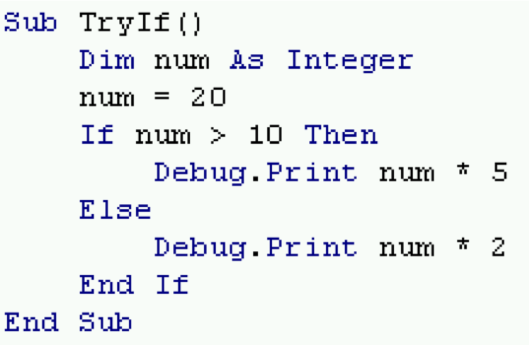
\includegraphics[width=0.4\textwidth]{img/Qcode}$$
\begin{multicols}{4}
\begin{enumerate}[A)]
\item 100
\item 40
\item 20
\item error
\end{enumerate}
\end{multicols}
\end{exampleblock}
\end{frame}


\begin{frame}[fragile]
\ft{Question: Decisions}
\begin{block}
{Question} What is the output of the following code:
$$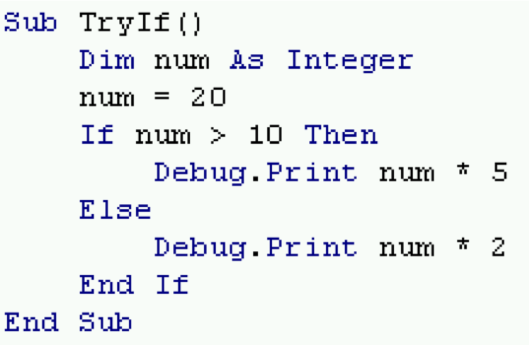
\includegraphics[width=0.4\textwidth]{img/Qcode}$$
\begin{multicols}{4}
\begin{enumerate}[A)]
\item \textbf<6>{\textit<6>{{\color<6>{iyellow}{100}}}}
\item 40
\item 20
\item error
\end{enumerate}
\end{multicols}
\end{block}
\end{frame}

\begin{frame}[t,fragile]
\ft{Try It: Decisions}
\begin{exampleblock}
{Question} Create a method called {\tt EchoDecision} that asks user a Yes and No question and outputs a message either {\tt "Yes"} or {\tt "No"} depending on what they chose.
\end{exampleblock}\pause
$$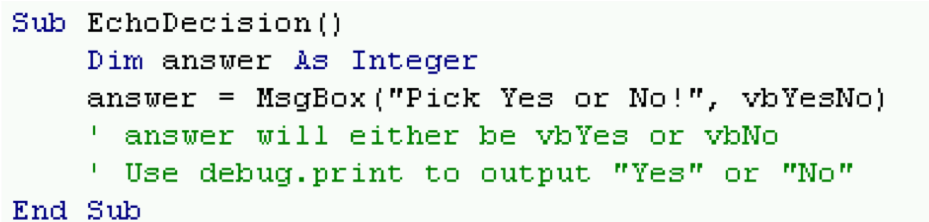
\includegraphics[width=0.9\textwidth]{img/trydecide}$$
\end{frame}





\begin{frame}[fragile]
\ft{Loops and Iteration}
A \emph{loop} repeats a set of statements multiple times until some condition is satisfied.\eol
Each time a loop is executed is called an \emph{iteration}.\eol
A \emph{{\tt for} loop} repeats statements a given number of times.

Example:
\begin{itemize}
\item 
\begin{verbatim}
Dim i as Integer
For i = 1 To 5
    Debug.Print i
Next i
\end{verbatim}
\end{itemize}
\end{frame}

\begin{frame}[fragile]
\ft{Question: loops}
\begin{exampleblock}
{Question} How many numbers are printed with this loop?
$$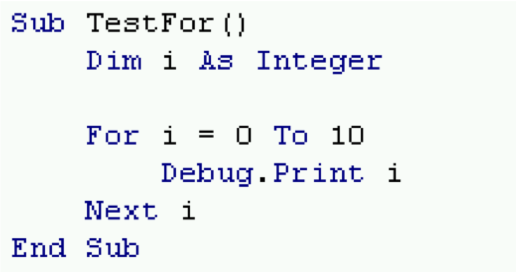
\includegraphics[width=0.4\textwidth]{img/printedloop}$$
\begin{multicols}{4}
\begin{enumerate}[A)]
\item 11
\item 10
\item 0
\item error
\end{enumerate}
\end{multicols}
\end{exampleblock}
\end{frame}


\begin{frame}[fragile]
\ft{Question: loops}
\begin{block}
{Question} How many numbers are printed with this loop?
$$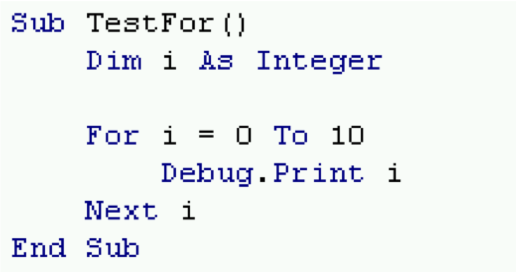
\includegraphics[width=0.4\textwidth]{img/printedloop}$$
\begin{multicols}{4}
\begin{enumerate}[A)]
\item \textbf<6>{\textit<6>{{\color<6>{iyellow}{11}}}}
\item 10
\item 0
\item error
\end{enumerate}
\end{multicols}
\end{block}
\end{frame}

\begin{frame}[fragile]
\ft{Try it: loops}
\begin{exampleblock}
{Homework:} Create a method called {\tt TryFor} that prints the numbers 1 to 20. \\[1em]
 Challenging variants:
\begin{enumerate}[a)]
\item Print the numbers from 10 down to 1.
\item Print only the even numbers from 1 to 10.
\end{enumerate}
\end{exampleblock}
\end{frame}

\begin{frame}[fragile]
\ft{User-Defined Functions (UDFs)}
A user-defined function is your own Excel function that can be used in formulas like built-in functions.\eol

A UDF must return a number, string, array, or Boolean.\eol

A UDF cannot change the Excel environment including the current cells or other cells (e.g. change formatting).\eol

Example: UDF doubleIt will double the input argument.
$$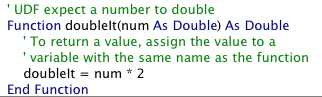
\includegraphics[width=0.8\textwidth]{img/UDF.png}$$
\end{frame}


\begin{frame}
\ft{UDF Example: Sum Cells by Background Colour}
$$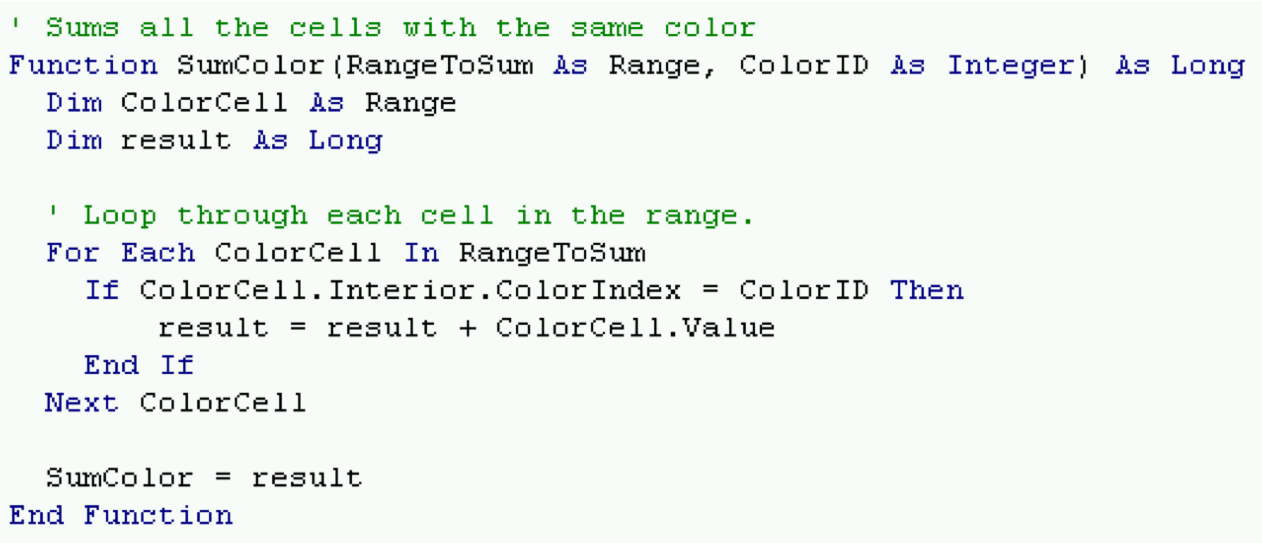
\includegraphics[width=0.9\textwidth]{img/UDFsum}$$
\begin{exampleblock}
{Question:}  Create a UDF called {\tt CountNum} that will return a count of the number of digits (0 to 9) in a string.
\end{exampleblock}
\end{frame}

\begin{frame}
\ft{Advanced: Object-Oriented Programming}
\emph{Object-oriented programming} structures code as objects, classes, methods, and properties.  This organization makes it easier to understand and construct large programs.\eol
An \emph{object} is an instance of a class that has its own properties and methods that define what the object is and what it can do.\eol
A \emph{class} is a generic template (blueprint) for creating an object.  All objects of a class have the same methods and properties (although the property values can be different).\eol
A \emph{property} is an attribute or feature of an object.\eol
A \emph{method} is a set of statements that performs an action.
\end{frame}

\begin{frame}[fragile]
\ft{Excel Objects}
Excel structures everything as a hierarchy of objects, and commands are done by running a method of an object.\eol
An object may contain other objects as well as methods and properties. \eol
A dot {\tt "."} is used as a separator between objects and subobjects, methods, and properties.\eol
Examples:
\begin{itemize}
 \item Top-level object: {\tt Application}
\item {\tt Workbook} -- individual Excel file
\item {\tt Worksheet} - sheet in a workbook
\end{itemize}

{\footnotesize \tt Application.ActiveWorkbook.Worksheets("macro").Range("A1").Value}
\end{frame}

\begin{frame}[fragile]
\ft{Excel Objects}
\begin{description}
\item[Range Object] The {\tt Range} object selects a cell or group of cells.
Example:
\begin{itemize}
\item {\tt Worksheets("Sheet1")}\\
 {\tt \orange{.Range("A1:C3")}.Font.Italic = True}\eol
\end{itemize}

\item[Object Methods] Methods perform an action.\\
Example:
\begin{itemize}
\item {\tt Worksheets("macro").Activate}
\end{itemize}
\end{description}
\end{frame}


\begin{frame}
\begin{exampleblock}{Question}
How many of the following statements are TRUE?
\begin{enumerate}
\item A method can have no parameters.
\item Two objects of the same class have the same properties.
\item Two objects of the same class may have different values for their properties.
\item Workbook is the top-level object in Excel.
\end{enumerate}
\begin{multicols}{5}
\begin{enumerate}[A)]
\item 0 
\item 1
\item 2
\item 3
\item 4
\end{enumerate}
\end{multicols}
\end{exampleblock}
\end{frame}



\begin{frame}
\begin{block}{Question}
How many of the following statements are TRUE?
\begin{enumerate}
\item {\color<2->{ForestGreen}{A method can have no parameters.}}
\item {\color<2->{ForestGreen}{Two objects of the same class have the same properties.}}
\item {\color<2->{ForestGreen}{Two objects of the same class may have different values for their properties.}}
\item {\color<2->{red}{Workbook is the top-level object in Excel.}}
\end{enumerate}
\begin{multicols}{5}
\begin{enumerate}[A)]
\item 0 
\item 1
\item 2
\item \textbf<6>{\textit<6>{{\color<6>{iyellow}{3}}}}
\item 4
\end{enumerate}
\end{multicols}
\end{block}
\end{frame}



\begin{frame}[fragile]
\ft{Try it: Excel Objects}
\begin{exampleblock}
{Question}Using the Immediate window try to perform the following actions with methods on Excel objects:
\begin{enumerate}
\item Switch the active worksheet to form.
\item Switch the active cell to macro sheet A4.
\item Use {\tt msgbox} to display value in current cell ({\tt ActiveCell}).
\end{enumerate}
\end{exampleblock}
\end{frame}




\begin{frame}[fragile]
\ft{Forms and Input Controls}
Excel allows the creation of forms with controls for a better interface.\eol

There are two types of controls in Excel:
\begin{enumerate}
\item Form controls -- default
\item ActiveX controls -- allow more flexibility and customization
\end{enumerate}

Controls can be inserted from the Developer tab. Select Insert, pick control, and then click and drag the size and shape of the control on the spreadsheet.

\end{frame}

\begin{frame}[fragile]
\ft{Input Controls}
$$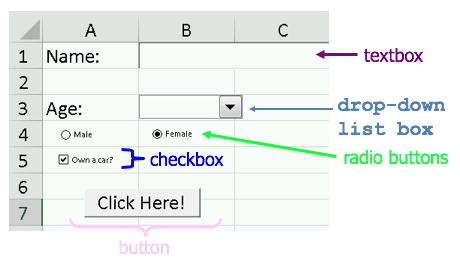
\includegraphics[width=0.8\textwidth]{img/InputControls.png}$$
\end{frame}

\begin{frame}[fragile]
\ft{Events}
An \emph{event} is a notification to your program that something has occurred.\eol
Events in Excel: 
\begin{itemize}
\item add a worksheet
\item double-click on a cell
\item change a cell value
\item calculating a formula
\item click on a button (can execute a macro)
\end{itemize}
Worksheet-level events on a particular worksheet and workbook level events for entire file.
\end{frame}

\begin{frame}[fragile]
\ft{Conclusion}
\emph{Microsoft Excel VBA} allows for automating tasks in Excel and provides a full programming environment for data analysis.\eol

\emph{Macros} record a set of actions so they can be easily executed again. \alert{Be aware of security risks when using macros.}\eol

The \emph{Visual Basic Editor (VBE)} is a complete integrated development environment for editing macros, \emph{user-defined functions}, and adding forms and controls that dynamically respond to events.\eol

Excel VBA uses \emph{object-oriented programming} that structures code as object, classes, methods, and properties.  A developer can control and automate everything with Excel using VBA.
\end{frame}

\begin{frame}[fragile]
\ft{Objectives}
\begin{itemize}
\item List some reasons to use Excel VBA
\item Define macro and explain the benefit of using macros
\item Be able to record and execute a macro
\item Explain the security issues with macros and how Excel deals with them
\item List and explain the use of the four main windows of the Visual Basic Editor
\item Explain the role of the object browser
\item Explain and use the WITH statement syntax
\item Be able to write simple macros using the VBE
\item Define: algorithm, program, language
\item Define: object-oriented programming, object, class, property, method
\item Understand and use dot-notation
\item Use the Range object to select a group of cells
\end{itemize}
\end{frame}

\begin{frame}[fragile]
\ft{Objectives (2)}
\begin{itemize}
\item Define: variable, value, location
\item Create and use Excel variables
\item Explain how a collection is different from a typical variable
\item Use If/Then/Else syntax to make decisions
\item Use For loop for repetition
\item Create user-defined functions and use them in formulas
\item Define: event
\item List some typical user interface controls
\item Understand that Excel allows for forms and controls to be added to a worksheet which respond to events
\end{itemize}
\end{frame}


\begin{frame}[label=current]
  {Questions}

  \nocite{lorem,ipsum}
  \bibliographystyle{plain}
  \bibliography{../demo}

\end{frame}

\end{document}

